\begin{Problem}
For each benchmark application, you need to report the dynamic counts and percentages of the following seventeen types of instructions. The total number of instructions (to be used as the denominator in the percentage) is the addition of all these seventeen counters. \\

% 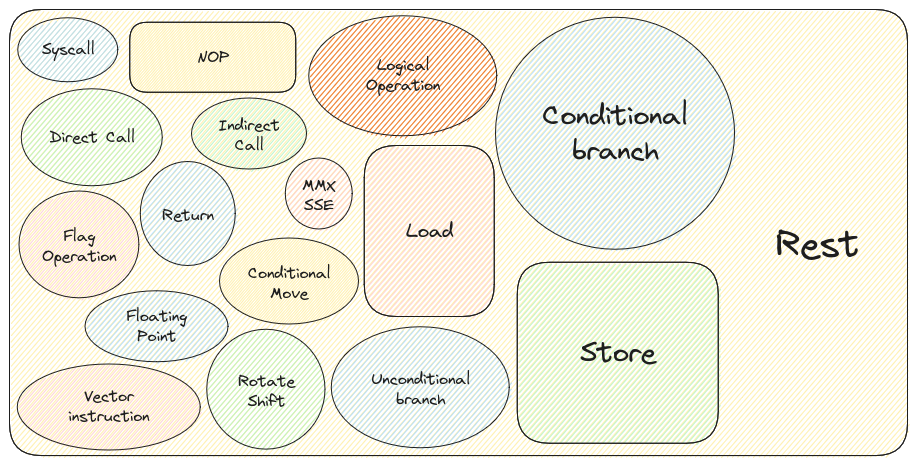
\includegraphics[width=0.9\textwidth]{./images/CS422_QuestionA.png}

Prepare a table showing these counts and percentages for the applications.
\end{Problem}

\begin{Solution}

\begin{figure}[H]
    \centering
    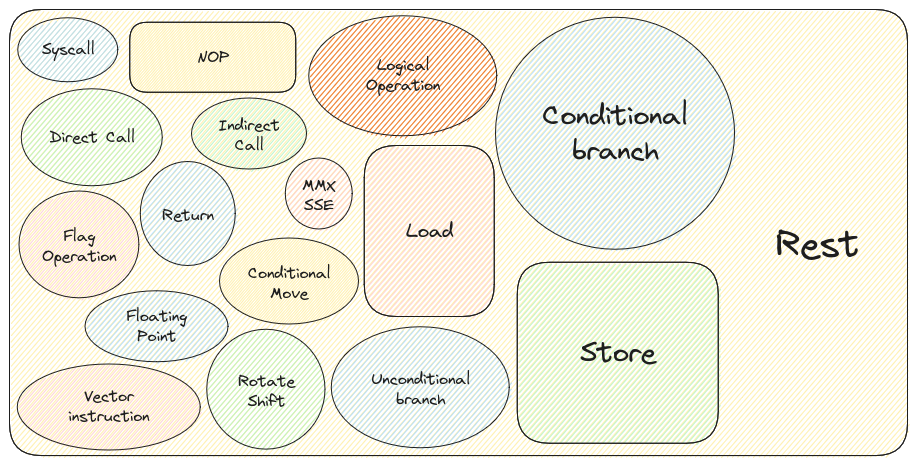
\includegraphics[width=0.9\textwidth]{images/CS422_QuestionA.png}
    \caption{Types of Instructions (Load-Store may overlap others)}
    \label{fig:pA:partitions}
\end{figure}

All the benchmark applications provided were fast-forwarded by a given number of instructions. During fast-forwarding, consider each instruction irrespective of type, as $1$ instruction while in instrumentation period, considered every instruction containing $n$ 32b loads and $m$ 32b stores components as equivalent to $1 + n + m$ instructions.

\vspace{10pt}
The below tables store the required data regarding all type of instructions. ``Percent" is the corresponding $\frac{\text{Count}}{\text{Effective}}$ where ``Effective" is as in \ref{tab:pA:instruction_counts}.

We found ``Vector Instructions", ``Conditional Moves", ``MMX and SSE Instructions", and ``System Calls" to be $0$ for all the applications.

Below at \ref{tab:pA:floating_rest_counts}, Memory Instructions is essentially Loads and Stores together.

\begin{table}[!htbp]
\centering
\caption{Actual \#Instruction v/s Effective $1 + n + m$ \#Instruction and their ratio}
\label{tab:pA:instruction_counts}
\begin{tabular}{| l | c | >{\columncolor[gray]{0.8}}c | >{\columncolor[gray]{0.8}}c | c |}
\hline
\multirow{2}{*}{Application} & \multirow{2}{*}{FastForward$^{(B)}$} & \multicolumn{2}{c|}{Instruction Counts} & \multirow{2}{*}{Percentage} \\
\cline{3-4}
& & Actual & Effective & \\
\hline
400.perlbench & 207 & 643629926 & 999864910 & 64.37\% \\
\hline
401.bzip2 & 301 & 626757711 & 999997068 & 62.67\% \\
\hline
403.gcc & 107 & 694478005 & 999992310 & 69.45\% \\
\hline
429.mcf & 377 & 660698717 & 1000000000 & 66.07\% \\
\hline
450.soplex & 364 & 615283889 & 1000000001 & 61.53\% \\
\hline
456.hmmer & 264 & 616007786 & 999999444 & 61.60\% \\
\hline
471.omnetpp & 43 & 625784586 & 1000000000 & 62.58\% \\
\hline
483.xalancbmk & 1331 & 652390226 & 999688603 & 65.26\% \\
\hline
\end{tabular}
\end{table}

\begin{table}[!htbp]
\centering
\caption{Load and Store \#Instructions}
\label{tab:pA:load_store_counts}
\begin{tabular}{| l | >{\columncolor[gray]{0.8}}c | c | >{\columncolor[gray]{0.8}}c | c |}
\hline
\multirow{2}{*}{Application} & \multicolumn{2}{c|}{Loads} & \multicolumn{2}{c|}{Stores} \\
\cline{2-3}\cline{4-5}
& Count & Percent & Count & Percent \\
\hline
400.perlbench & 235396718 & 23.543 & 120973356 & 12.099 \\
\hline
401.bzip2 & 286663856 & 28.666 & 86578433 & 8.658 \\
\hline
403.gcc & 22555350 & 2.255 & 282966645 & 28.301 \\
\hline
429.mcf & 274762679 & 27.476 & 64538604 & 6.459 \\
\hline
450.soplex & 335145819 & 33.514 & 49570293 & 4.957 \\
\hline
456.hmmer & 337431712 & 33.743 & 46560502 & 4.656 \\
\hline
471.omnetpp & 232166088 & 23.217 & 142049326 & 14.205 \\
\hline
483.xalancbmk & 239302390 & 23.938 & 108307384 & 10.834 \\
\hline
\end{tabular}
\end{table}

\begin{table}[!htbp]
\centering
\caption{NOP, Direct and Indirect Calls \#Instructions}
\label{tab:pA:nop_calls_counts}
\begin{tabular}{| l | >{\columncolor[gray]{0.8}}c | c | >{\columncolor[gray]{0.8}}c | c | >{\columncolor[gray]{0.8}}c | c |}
\hline
\multirow{2}{*}{Application} & \multicolumn{2}{c|}{NOPs} & \multicolumn{2}{c|}{Direct Calls} & \multicolumn{2}{c|}{Indirect Calls} \\
\cline{2-3}\cline{4-5}\cline{6-7}
& Count & Percent & Count & Percent & Count & Percent \\
\hline
400.perlbench & 433528 & 0.0433 & 6947662 & 0.695 & 2165028 & 0.216 \\
\hline
401.bzip2 & 32147 & 0.00321 & 11032 & 0.00110 & 0 & 0.000 \\
\hline
403.gcc & 90112 & 0.00901 & 1275299 & 0.128 & 13555 & 0.00136 \\
\hline
429.mcf & 879752 & 0.0879 & 8266384 & 0.826 & 0 & 0.000 \\
\hline
450.soplex & 1852 & 0.00018 & 2374689 & 0.237 & 54 & 0.0000 \\
\hline
456.hmmer & 14312 & 0.0014 & 86688 & 0.0087 & 553 & 0.00005 \\
\hline
471.omnetpp & 503202 & 0.0503 & 13391515 & 1.339 & 2307982 & 0.231 \\
\hline
483.xalancbmk & 14237079 & 1.424 & 8707590 & 0.871 & 5826909 & 0.583 \\
\hline
\end{tabular}
\end{table}

\begin{table}[!htbp]
\centering
\caption{Returns, Unconditional and Conditional Branches \#Instructions}
\label{tab:pA:ret_branch_counts}
\begin{tabular}{| l | >{\columncolor[gray]{0.8}}c | c | >{\columncolor[gray]{0.8}}c | c | >{\columncolor[gray]{0.8}}c | c |}
\hline
\multirow{2}{*}{Application} & \multicolumn{2}{c|}{Returns} & \multicolumn{2}{c|}{Uncond. Branches} & \multicolumn{2}{c|}{Cond. Branches} \\
\cline{2-3}\cline{4-5}\cline{6-7}
& Count & Percent & Count & Percent & Count & Percent \\
\hline
400.perlbench & 9112689 & 0.911 & 20172634 & 2.017 & 82678603 & 8.268 \\
\hline
401.bzip2 & 11031 & 0.0011 & 14741341 & 1.474 & 84526720 & 8.453 \\
\hline
403.gcc & 1288855 & 0.128 & 1488031 & 0.148 & 97945541 & 9.794 \\
\hline
429.mcf & 8266383 & 0.826 & 5572158 & 0.557 & 117749486 & 11.77 \\
\hline
450.soplex & 2374743 & 0.237 & 7571500 & 0.757 & 64241385 & 6.424 \\
\hline
456.hmmer & 87241 & 0.0087 & 113915 & 0.0113 & 88919715 & 8.891 \\
\hline
471.omnetpp & 15699500 & 1.569 & 13881657 & 1.388 & 73391837 & 7.339 \\
\hline
483.xalancbmk & 14538758 & 1.454 & 5687717 & 0.568 & 115456999 & 11.549 \\
\hline
\end{tabular}
\end{table}

\begin{table}[H]
\centering
\caption{Logical, Rotate-Shift and Flag Operations \#Instructions}
\label{tab:pA:logic_flag_counts}
\begin{tabular}{| l | >{\columncolor[gray]{0.8}}c | c | >{\columncolor[gray]{0.8}}c | c | >{\columncolor[gray]{0.8}}c | c |}
\hline
\multirow{2}{*}{Application} & \multicolumn{2}{c|}{Logical Op} & \multicolumn{2}{c|}{Rotate \& Shift} & \multicolumn{2}{c|}{Flag Op} \\
\cline{2-3}\cline{4-5}\cline{6-7}
& Count & Percent & Count & Percent & Count & Percent \\
\hline
400.perlbench & 61151842 & 6.116 & 2897866 & 0.289 & 478094 & 0.0478 \\
\hline
401.bzip2 & 51058392 & 5.105 & 44677195 & 4.467 & 4398 & 0.0004 \\
\hline
403.gcc & 94626225 & 9.462 & 917464 & 0.0917 & 36715 & 0.0036 \\
\hline
429.mcf & 49278688 & 4.927 & 2313100 & 0.231 & 0 & 0.000 \\
\hline
450.soplex & 8780117 & 0.878 & 6691975 & 0.669 & 13408915 & 1.340 \\
\hline
456.hmmer & 692045 & 0.0692 & 167329 & 0.0167 & 2879 & 0.0002 \\
\hline
471.omnetpp & 37629094 & 3.762 & 4483798 & 0.448 & 12598264 & 1.259 \\
\hline
483.xalancbmk & 24767577 & 2.477 & 3702529 & 0.370 & 1093111 & 0.109 \\
\hline
\end{tabular}
\end{table}

\begin{table}[H]
\centering
\caption{Floating Point, Rest of Instructions, and Total Memory Operations \#Instructions}
\label{tab:pA:floating_rest_counts}
\begin{tabular}{| l | >{\columncolor[gray]{0.8}}c | c | >{\columncolor[gray]{0.8}}c | c | >{\columncolor[gray]{0.8}}c | c |}
\hline
\multirow{2}{*}{Application} & \multicolumn{2}{c|}{Floating Point} & \multicolumn{2}{c|}{The Rest} & \multicolumn{2}{c|}{Memory Instructions} \\
\cline{2-3}\cline{4-5}\cline{6-7}
& Count & Percent & Count & Percent & Count & Percent \\
\hline
400.perlbench & 342346 & 0.0342 & 457114544 & 45.717 & 351643026 & 35.169 \\
\hline
401.bzip2 & 0 & 0.000 & 431692523 & 43.169 & 371409789 & 37.141 \\
\hline
403.gcc & 0 & 0.000 & 496788518 & 49.679 & 305508440 & 30.551 \\
\hline
429.mcf & 0 & 0.000 & 468372766 & 46.837 & 339301283 & 33.930 \\
\hline
450.soplex & 186666057 & 18.666 & 323172602 & 32.317 & 291902950 & 29.190 \\
\hline
456.hmmer & 17169 & 0.00171 & 525905384 & 52.590 & 383971218 & 38.397 \\
\hline
471.omnetpp & 60608252 & 6.060 & 391289485 & 39.128 & 344614207 & 34.461 \\
\hline
483.xalancbmk & 4770381 & 0.477 & 453290179 & 45.343 & 330430323 & 33.053 \\
\hline
\end{tabular}
\end{table}

\end{Solution}